\documentclass{beamer}
\usetheme{Madrid}
\usecolortheme{dolphin}
\useoutertheme{smoothbars}
\usepackage{listings}
\usepackage{xcolor}
\usepackage{tikz}
\usepackage{booktabs} % 表格更專業
\usetikzlibrary{positioning, arrows.meta}




% 設定 R 語言的程式碼格式
\lstset{
    language=R,
    basicstyle=\ttfamily\small,
    keywordstyle=\color{blue},
    commentstyle=\color{gray},
    stringstyle=\color{red},
    breaklines=true,
    showstringspaces=false,
    frame=single
}

% 加入點點導航條
\setbeamertemplate{headline}{
  \begin{beamercolorbox}[ht=2.5ex,dp=1ex,left]{section in head/foot}
    \hspace{1em} \insertsectionnavigationhorizontal{\textwidth}{}{}
  \end{beamercolorbox}
}

\author{Yuze Tsai}
\title{Machine Learning Project}
\subtitle{Approach for Investigating the Impact of Circular Economy on Taiwan's Economy and the Energy efficiency}

\begin{document}

    \frame {
        \titlepage
    }

    % 目錄頁
    \frame {
        \frametitle{Table of Contents}
        \tableofcontents
    }

    % 第一個章節
    \section{Introduction}
    \frame {
        \frametitle{Introduction}
        \begin{itemize}
        \item What is Circular Economy?
        \item Why this topic important?
        \end{itemize}
        \begin{figure}[H]
            \centering
            
\includegraphics[width=0.5\linewidth]{/Users/yuzetsai/Desktop/untitled_folder/sustainability-10-02141-g001.png}
            \label{fig:enter-label}
        \end{figure}
    }

    \frame{
        \frametitle{References}
        \framesubtitle{Variables of interest}
        \begin{itemize}
            \item Tanatu, A., et al.(2018): Resource productivity and domestic material consumption has a strong relationship
            with municipal waste recycling,
            \item The Ex’TAX project (2022) study: Taxshift can accelerate the transition to circular in construction industry
            \item Radivojevi´c, V, et al.(2024): A strong positive correlation between circular economy indicators and GDP per capita.
        \end{itemize}
    }

    % 其他章節
    \section{Data Collections}
    \frame{
        \frametitle{What we have right now...}
        \begin{itemize}
            \item \textbf{Dependent Variables}: Total city/county income, Per capita electricity consumption, Vacancy Rates of House
            \item \textbf{Independent and Policy-Related Variables} Water pollution environmental tax, Air pollution environmental tax, General waste recycling rate...(total = 11)
            \item \textbf{Year of Interest}: 2014 - 2023 (10 years)
        \end{itemize}
       
    }
    \frame{
        \frametitle{Data Manipualtion}
        \begin{figure}[H]
            \centering
            \includegraphics[width=\textwidth]{/Users/yuzetsai/Desktop/untitled folder/Screenshot 2025-03-31 at 4.03.57 pm.png}
            \label{fig:enter-label}
        \end{figure}     
    }
    \frame{
        \frametitle{Data Manipualtion}
        \begin{figure}[H]
            \centering
            \includegraphics[width=\textwidth]{/Users/yuzetsai/Desktop/Screenshot 2025-04-01 at 9.14.58 am.png}
            \label{fig:enter-label}
        \end{figure}     
    }

    \section{Methods}
    \begin{frame}{Flow Chart of Study Structure}
        \centering
        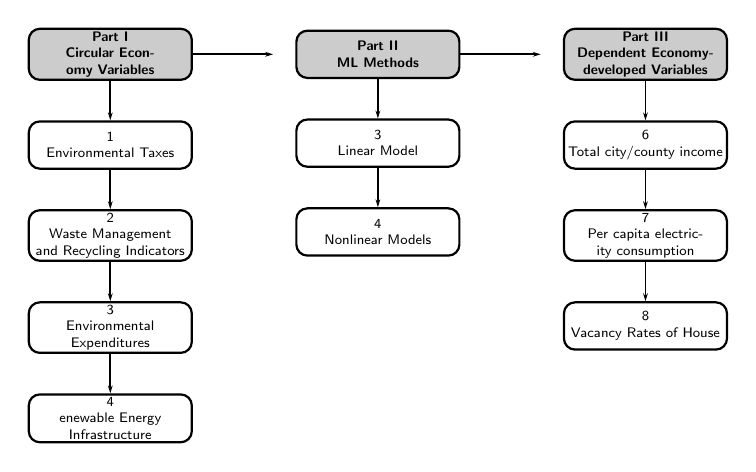
\begin{tikzpicture}[
            block/.style={rectangle, rounded corners, minimum height=6mm, minimum width=20mm, 
                          text width=20mm, align=center, thick, font=\sffamily\tiny, inner sep=1pt}, 
            node distance=0.3cm % Increase vertical spacing
        ]
        
            % Part I
            \node[draw, fill=gray!40, block] (s) at (-1,0) {\textbf{Part I \\ Circular Economy Variables}};
            \node[draw, block, below=of s, yshift=-2mm] (s1) {1 \\ Environmental Taxes};
            \node[draw, block, below=of s1, yshift=-2mm] (s2) {2 \\ Waste Management and Recycling Indicators};
            \node[draw, block, below=of s2, yshift=-2mm] (s3) {3 \\ Environmental Expenditures};
            \node[draw, block, below=of s3, yshift=-2mm] (s4) {4 \\ enewable Energy Infrastructure};
            \draw[-{Stealth[length=1mm, width=0.6mm]}, semithick] (s.south) -- (s1.north);
            \draw[-{Stealth[length=1mm, width=0.6mm]}, semithick] (s1.south) -- (s2.north);
            \draw[-{Stealth[length=1mm, width=0.6mm]}, semithick] (s2.south) -- (s3.north);
            \draw[-{Stealth[length=1mm, width=0.6mm]}, semithick] (s3.south) -- (s4.north);
            % Part II
            \node[draw, fill=gray!40, block, right=of s, xshift=1cm] (a) {\textbf{Part II \\ ML Methods}};
            \node[draw, block, below=of a, yshift=-2mm] (a1) {3 \\ Linear Model};
            \node[draw, block, below=of a1, yshift=-2mm] (a2) {4 \\ Nonlinear Models};
            \draw[-{Stealth[length=1mm, width=0.6mm]}, semithick] (a.south) -- (a1.north);
            \draw[-{Stealth[length=1mm, width=0.6mm]}, semithick] (a1.south) -- (a2.north);

    
            % Part III
            \node[draw, fill=gray!40, block, right=of a, xshift=1cm] (b) {\textbf{Part III \\ Dependent Economy-developed Variables}};
            \node[draw, block, below=of b, yshift=-2mm] (b1) {6 \\ Total city/county income};
            \node[draw, block, below=of b1, yshift=-2mm] (b2) {7 \\ Per capita electricity consumption};
            \node[draw, block, below=of b2, yshift=-2mm] (b3) {8 \\ Vacancy Rates of House};
            \draw[-{Stealth[length=1mm, width=0.6mm]}, semithick] (b.south) -- (b1.north);
            \draw[-{Stealth[length=1mm, width=0.6mm]}, semithick] (b1.south) -- (b2.north);
            \draw[-{Stealth[length=1mm, width=0.6mm]}, semithick] (b2.south) -- (b3.north);
            
    
            % Shortened Horizontal Arrows (more)
            \draw[-{Stealth[length=1mm, width=0.6mm]}, semithick, shorten >= 8pt] (s.east) -- (a.west);
            \draw[-{Stealth[length=1mm, width=0.6mm]}, semithick, shorten >= 8pt] (a.east) -- (b.west);

    
        \end{tikzpicture}
    \end{frame}
    \frame{
        \frametitle{Linear Regression Method -- Panel Data Regression}
        
        \begin{equation}
            y_{it} = a + X^\prime_{it} \beta + c_{i} + e_{it}
        \end{equation}
        
        where we define:  
        \begin{itemize}
            \item \( i = 1, \dots, N \), where \( i \) represents a county/city, and we have \( N \) cross-sectional data (\( N = 22 \)).
            \item \( t = 2013, \dots, 2023 \).
            \item \( y_{it} \) is the dependent variable.
            \item \( X^\prime_{it} \) are the independent variables of \( K \)-dimension.
            \item \( a \) is the intercept.
            \item \( \beta \) is the coefficient vector of \( K \)-dimension.
            \item \( c_{i} \) is the individual effect.
            \item \( e_{it} \) is the error term.
        \end{itemize}
    }
    \begin{frame}{Fixed Effects vs. Random Effects}
        \centering
        \scriptsize % 讓表格更小
        \begin{tabular}{lcc}
            \toprule
            \textbf{Feature} & \textbf{Fixed Effects (FE)} & \textbf{Random Effects (RE)} \\
            \midrule
            Individual Effect \( c_i \) & Fixed (correlated with \( X_{it} \)) & Random (uncorrelated) \\
            Main Assumption & Controls for time-invariant differences & Individual effects are uncorrelated \\
            Interpretation & Within-group variation & Between and within variation \\
            When to Use & If \( c_i \) is correlated with \( X_{it} \) & If \( c_i \) is random and uncorrelated \\
            \bottomrule
        \end{tabular}
        \begin{figure}[H]
            
\includegraphics[width=5cm]{/Users/yuzetsai/Desktop/demeaned.png}
        \end{figure}  
    \end{frame}

    \begin{frame}{Panel Data Model Selection}
        \centering
        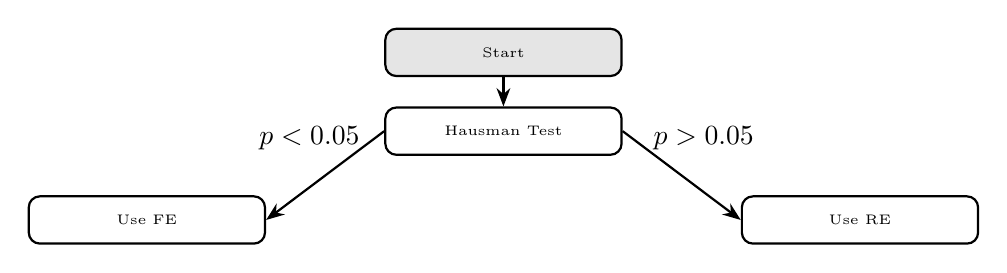
\begin{tikzpicture}[
            node distance=1cm and 1.5cm, % 縮小距離
            block/.style={rectangle, draw, rounded corners, minimum height=6mm, minimum width=30mm, font=\tiny, align=center, thick}
        ]
            \node[block, fill=gray!20] (start) {Start};
            \node[block, below of=start] (test) {Hausman Test};
            \node[block, below left=0.5cm and 1.5cm of test] (fe) {Use FE};
            \node[block, below right=0.5cm and 1.5cm of test] (re) {Use RE};
            

            \draw[-{Stealth}, thick] (start.south) -- (test.north);
            \draw[-{Stealth}, thick] (test.west) -- (fe.east) node[midway, above, yshift =0.2cm, xshift = -0.2cm] {\( p < 0.05 \)};
            \draw[-{Stealth}, thick] (test.east) -- (re.west) node[midway, above, yshift =0.2cm, xshift = 0.28cm] {\( p > 0.05 \)};
        \end{tikzpicture}
    \end{frame}
    
        

    \begin{frame}{Nonlinear regression method -- XGBoost}
        XGBoost (Extreme Gradient Boosting) is an ameliorated gradient boosting method that efficiently handles large datasets and has performed exceptionally well in many competitions.
        \begin{itemize}
            \item Uses \textbf{gradient boosting} to iteratively minimize errors.
        \end{itemize}

        \textbf{Mathematical Model:}
        \[
            \text{Loss} = \sum_{i=1}^{N} l(y_i, \hat{y}_i) + \sum_{k=1}^{K} \Omega(f_k)
        \]
        where:
        \begin{itemize}
            \item The first term represents prediction error.
            \item The second term is a regularization term controlling model complexity.
        \end{itemize}
        \vspace{0.3cm}
        \textbf{Pros and Cons:}  
        \begin{itemize}
            \item \textcolor{green}{Pros:} High accuracy, fast training.
            \item \textcolor{red}{Cons:} Complex parameter tuning.
        \end{itemize}
    \end{frame}

    \begin{frame}{Nonlinear regression method -- Random Forest}
        Random Forest is an \textbf{ensemble learning} method consisting of multiple decision trees. The final prediction is based on \textbf{voting (classification)} or \textbf{averaging (regression)}.
        \vspace{0.3cm}

        \vspace{0.3cm}
        \textbf{Pros and Cons:}  
        \begin{itemize}
            \item \textcolor{green}{Pros:} Handles high-dimensional data, reduces overfitting.
            \item \textcolor{red}{Cons:} Long training time, less interpretable.
        \end{itemize}
        \begin{figure}[H]
            \centering
            \includegraphics[width=5cm]{/Users/yuzetsai/Desktop/1678715398600.jpeg}
            \label{fig:enter-label}
        \end{figure}  
    \end{frame}
    \frame{
        \frametitle{Boosting vs Bagging}
        \begin{figure}[H]
            \centering
            \includegraphics[width=\textwidth]{/Users/yuzetsai/Desktop/1*_UIUphtL_vXJFeQ6vdKlCA.png}
        \end{figure}     
    }

    \begin{frame}{Nonlinear regression method -- Support Vector Machine (SVM)}
    SVM is a supervised learning algorithm primarily used for classification.  
        \begin{itemize}
            \item It finds the \textbf{optimal hyperplane} that best separates different classes.
            \item Uses \textbf{kernel functions} to handle non-linear classification.
        \end{itemize}
        \vspace{0.3cm}
        \textbf{Mathematical Formulation:}  
        \[
            \max_{\mathbf{w}, b} \quad \frac{1}{\|\mathbf{w}\|} 
        \]
        \[
            \text{subject to} \quad y_i (\mathbf{w} \cdot \mathbf{x}_i + b) \geq 1, \quad \forall i
        \]
        \vspace{0.3cm}
        \textbf{Pros and Cons:}  
        \begin{itemize}
            \item \textcolor{green}{Pros:} Effective in small sample, high-dimensional data.
            \item \textcolor{red}{Cons:} Computationally expensive, slow for large datasets.
        \end{itemize}
    \end{frame}
    \begin{frame}{Comparison of ML Methods}
        \begin{table}[]
            \centering
            \begin{tabular}{lccc}
                \toprule
                Feature & SVM & Random Forest & XGBoost \\
                \midrule
                Speed & Slow & Medium & Fast \\
                Accuracy & High & High & Very High \\
                Interpretability & Low & Medium & Low \\
                Handles Large Data & No & Yes & Yes \\
                \bottomrule
            \end{tabular}
        \end{table}
    \end{frame}
    
    \section{Expected Results}
    \frame{
        \frametitle{Intuitive Clairvoyance...}
        \begin{itemize}
            \item Environmental budgets and recycling efforts have a positive relationship with total income of a city.
            \item Cities that invested more in renewable energy infrastructure will generate some critical improvements in energy efficiency.
            \item Higher levels of incineration and landfill usage are associated with lower energy efficiency, possibly due to poor recycling practices.
        \end{itemize}
    }

\begin{frame}{Hausman Test for Model Selection}
    \begin{itemize}
        \item Null Hypothesis: \( H_0 : \mathbb{E}(c_i | X_{it}) = 0 \Rightarrow \) Random Effects (RE)
        \item Alternative Hypothesis: \( H_1 : \mathbb{E}(c_i | X_{it}) \neq 0 \Rightarrow \) Fixed Effects (FE)
        \item Based on the Hausman test, FE model is chosen if \( p < 0.05 \), suggesting correlation between individual effects and regressors.
        \item In this study, FE models are generally preferred due to practical data nature.
    \end{itemize}
\end{frame}

\section{Model Evaluation and Interpretation}
\begin{frame}{Model Evaluation and Comparison}
    \begin{itemize}
        \item \textbf{Performance Metrics:}
            \begin{itemize}
                \item Mean Squared Error (MSE)
                \item R-Squared (R²)
                \item Cross-validation (10-fold)
            \end{itemize}
        \item \textbf{Findings:}
            \begin{itemize}
                \item Nonlinear models generally outperform linear ones.
                \item CatBoost achieved the highest R² for household income and vacancy rate.
                \item SVM showed poor predictive performance; excluded from SHAP analysis.
            \end{itemize}
    \end{itemize}
\end{frame}

\begin{frame}{SHAP (SHapley Additive Explanations)}
    \begin{itemize}
        \item SHAP assigns each feature an importance value for prediction.
        \item Based on cooperative game theory—accounts for all possible feature combinations.
        \item \textbf{Advantages:}
            \begin{itemize}
                \item Global and local interpretability
                \item Indicates both direction (+/−) and magnitude of effect
                \item Helps identify nonlinear thresholds and interactions
            \end{itemize}
        \item \textbf{Applied to:} XGBoost, CatBoost, LightGBM, Random Forest
    \end{itemize}
\end{frame}


    
\end{document}
